\hypersetup{colorlinks=true, linkcolor=blue, citecolor=red}

\chapter{Preliminaries} \label{chap:preliminaries}

\section{Search Problems}

As briefly discussed in the introduction, the concept of \textbf{functional problems} rose as a generalization of the concept of decision problems. Mathematically, each decision problem can be defined as a subset of possible inputs: an input object is part of the set if and only if it has the required property. For example, the decision problem \say{is this number prime?} can be described as the set $\mathrm{PRIMES} = \{n \in \N \mid n \text{ is prime}\}$.

In a very similar way, functional problems can be described mathematically described through the concept of relation: given the set of inputs $X$ and the set of outputs $Y$ of the functional problem, the latter can be described as the relation $R \subseteq X \times Y$. An important thing to notice is that even though the name implies a correlation to mathematical functions, the given definition also includes partial and multi-valued functions, that being functions for which not all inputs have a corresponding output and functions for which one input can have more outputs.

For these reasons, the term \textit{functional problem} is considered to be slightly abused. In recent years, this issue was solved by the introduction of the term \textbf{search problems}, which describes problems based on finding an output for the given input. It's easy to see that this informal definition of search problems better suits the previous definition given for functional problems. While decision problems focus on answering the question \say{does this object have the following property?}, search problems focus on answering the question \say{what gives this object the following property?}. Mathematically, this can be described as the difference between \say{is there an output?} and \say{what is the output?}.For example, the search problem equivalent of the previous prime number problem would answer the question \say{what is the prime factorization of this number?}. 

We give a more detailed definition of each search problems through the use of a \textit{sequence of relations} rather than a single relation in order to allow inputs of different length and different types of outputs based on the length of the inputs. This definition is a conjunction of the various definitions given in \cite{search_problems_dt_model, rel_comp_np_search, proofs_circuits_communication, tfnp_characterization}.

\newpage

\begin{definition}
    A search problem is a sequence $R = (R_n)_{n \in \N}$ of relations $R_n \subseteq \{0,1\}^n \times O_n$, one for each $n \in \N$, where each $O_n$ is a finite set called "outcome set".

    A search problem is said to be total if for each $R_n$ in the sequence it holds that $\forall x \in \{0,1\}^n$ there is an $y \in O_n$ such that $(x,y) \in R_n$.
\end{definition}

In particular, this work will focus on \textbf{total search problems}. Notice that this definition removes partial function from the context, while multi-valued functions are still allowed. Moreover, complexity theory focuses on the study of \textbf{decidable} decision and search problems, that being problems for which we know that there is always an computable answer.

\quad

\section{The complexity classes \textsf{FP}, \textsf{FNP} and \textsf{TFNP}}

In complexity theory, decidable decision problems are grouped in two major classes: problems that can be \textbf{solved} in a reasonable amount of time and problems that can be \textbf{verified} in a reasonable amount of time. These classes are respectively referred to as \textsf{P}, the class of problems solvable by a deterministic algorithm in polynomial time, and \textsf{NP}, the class of problems for which a solution can be verified by a a deterministic algorithm in polynomial time (or equivalently, the class of problems solvable by a non-deterministic algorithm). By the very definition of these classes, it's easy to see that \textsf{P} $\subseteq$ \textsf{NP}. 

Similarly, in the context of search problems we define the classes \textsf{FP} and \textsf{FNP}, standing for \textit{functional \textsf{P}} and \textit{functional \textsf{NP}}. An important remark to be made is that, since they are defined on two different types of problems, it doesn't hold that \textsf{P} $\subseteq$ \textsf{FP} or that \textsf{NP} $\subseteq$ \textsf{FNP}. However, a decision problem can indeed be seen as a search problem with only two different outputs: \textit{true} or \textit{false}. In fact, as discussed in \cite{decision_vs_search, rel_comp_np_search, fp_vs_p}, an important result is that $\textsf{P} = \textsf{NP} $ if and only if $\textsf{FP} = \textsf{FNP}$, meaning that even though search problems are generally harder than decision problems, even if the latter are efficiently solvable then the other also is.

Moreover, by the very own nature of search problems, it's important to distinct between \textit{total} and \textit{partial} search problems. Thus, for search problems we also define the class \textsf{TFNP}, standing for \textit{total functional \textsf{NP}}.

\begin{definition}
    A search problem $R$ is in \textsf{FP} if it is solvable by an algorithm in polynomial time. Likewise, as search problem $R$ is in \textsf{FNP} if its solutions are verifiable by an algorithm in polynomial time. If the search problem is also total, it is in \textsf{TFNP}.
\end{definition}

Additionally, we will assume that each problem in \textsf{FP} is also total: since problems in \textsf{FP} are \textit{solvable} in polynomial time, when a solution doesn't exist for a given input we can consider the solution to be a pre-chosen \say{doesn't exist} value, making the problem total. Obviously, this assumption implies that \textsf{FP} $\subseteq$ \textsf{TFNP} $\subseteq$ \textsf{FNP}. 

Differently from decision problems, search problems are conjectured to not have any "normal" complete problem, that being problems for which an efficient solution would imply an efficient solution for any other search problem. The reason behind this conjecture is the nature itself of total search problems: in decision problems, any "yes" (or "no") answer can be reduced to a "yes" (or "no) answer of a complete decision problem, but total search problems imply that every input has a "yes" instance as output, meaning that there is no way for an instance to be reduced to another "no" instance.

For these reasons, for search problems we define the concept of completeness with respect to a \textbf{specific search problem}: given a search problem $R$, we define the subclass of all search problems reducible to $R$. Thus, the problem $R$ is said to be "complete" for its own class of reducible problems. Unexpectedly, a lot of \textsf{TFNP} problems can be characterized with very few cases of such subclasses, giving birth to an actual hierarchy of search problems.

\begin{figure}[H]
    \centering
    
    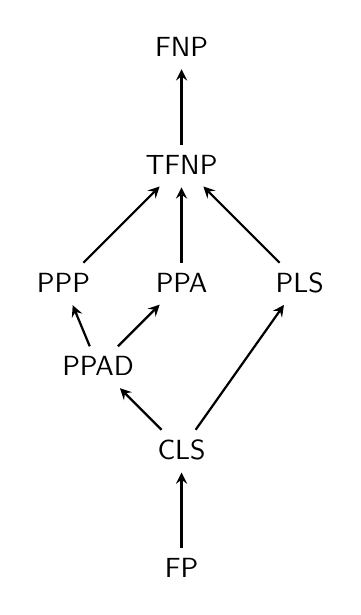
\begin{tikzpicture}[->,>=stealth,shorten >=1pt,auto,node distance=1.5cm, thick,main node/.style={scale=0.9,circle,draw,font=\sffamily\normalsize}]
    
        \node (1) []{\textsf{FNP}};

        \node (2) [below of = 1]{\textsf{TFNP}};

        \node (3) [below of = 2]{\textsf{PPA}};

        \node (4) [left of = 3]{\textsf{PPP}};

        \node (5) [right of = 3]{\textsf{PLS}};

        \node (6) [below left of = 3]{\textsf{PPAD}};

        \node (7) [below right of = 6]{\textsf{CLS}};

        \node (8) [below of = 7]{\textsf{FP}};
    
        \path[every node/.style={font=\sffamily\small}]
            (8) edge (7)
            (7) edge (6)
            (7) edge (5)
            (6) edge (4)
            (6) edge (3)
            (5) edge (2)
            (4) edge (2)
            (3) edge (2)
            (2) edge (1)
        ;
    \end{tikzpicture}
    
    \caption{Hierarchy of the most commonly defined complete search problem classes. An arrow from class $A$ to class $B$ means that $A \subseteq B$.}
\end{figure}

Each of the subclasses shown in the previous hierarchy is characterized by a \textbf{complete search problem}:
\begin{itemize}
    \item \textsf{PPP} (Polynomial Pigeonhole Principle): the class of problems whose solution is guaranteed by the Pigeonhole principle. It is defined as the class of problems that are polynomial-time reducible to the \textit{Pigeon problem}
    
    
    \item \textsf{PPA} (Polynomial Parity Argument): is the class of problems whose solution is guaranteed by the handshaking lemma. It is defined as the class of problems that are polynomial-time reducible to the \textit{Odd-degree Vertices problem}.
    
    \item \textsf{PLS} (Polynomial Local Search): the class of search problems designed to model the process of finding a local optimum of a function. It is defined as the class of problems that are polynomial-time reducible to the \textit{Sink-of-DAG problem}.
    
    \item \textsf{PPAD} (Polynomial Parity Argument - Directed): is the class of problems whose solution is guaranteed by the directed version of the handshaking lemma. It is defined as the class of problems that are polynomial-time reducible to the \textit{End-of-Line problem}.
    
    \item \textsf{CLS} (Continuous Local Search): the class of search problems designed to model the process of finding a local optimum of a continuous function over a continuous domain. It is defined as the class of problems that are polynomial-time reducible to the \textit{Continuous Localpoint problem}.
\end{itemize}

Proving any separation between one of these inclusions would directly conclude that \textsf{FP} $\neq$ \textsf{FNP}, giving an answer to the conjecture.
 
\newpage

\section{Proof Complexity}

\section{Communication Complexity}

\section{Circuit Complexity}

\cleardoublepage